\section{Theoretische Grundlagen}
Um in Seminarräumen, Hörsälen oder Klassenzimmer das Risiko von einer Vireninfektion gering zu halten, ist eine gute Durchlüftung des jeweiligen Raumes nötig. Wie oft gelüftet werden sollte hängt von mehreren Parametern ab, welche sich gerade für Aerosole als kompliziert erweisen. \\
Hierbei werden Modelle für die Tröpfchenbildung, deren Sinkgeschwindigkeit, sowie Effizienz der Masken und ähnliches zurate gezogen. \\
Um dennoch eine sinnvolle Belüftung von Räumlichkeiten zu gewährleisten, können bereits untersuchte Luftparameter wie der CO2-Gehalt in Arbeitsräumen genutzt werden. Für diese Annahme wird davon ausgegangen, dass je mehr CO¬2 sich in der Luft befindet, desto höher ist das Risiko, dass bereits ausgeatmete Luft zusammen mit Aerosolen wieder eingeatmet wird. \\
Über den CO2-Gehalt kann somit eine indirekte Messung an Aerosolen erfolgen und entsprechende Messgeräte wie CO2-Ampeln auf ein Mindestmaß an Lüftung hinweisen.\\
Doch wie lässt sich nun der CO2-Gehalt in einem Raum bestimmen? Welche Kriterien für die maximale Konzentration sollen dabei eingehalten werden? \cite{Hartmann.2020,Simmank.15.08.2020,bghm2020}

\subsection{Die Pettenkofer-Zahl}
Prof. Max Pettenkofer (1818-1901) definierte bereits 1858 eine anzustrebende Obergrenze für den \ce{CO2}-Gehalt in einem Raum von 1000 ppm = 0,10 Vol.\%. Dieser Grenzwert ist auch heute noch als \textsc{Pettenkofer}-Zahl bekannt.
Entstanden aus der Zeit der Industrialisierung und als technische Regel an Arbeitsstätten hinzugezogen, beweist sich auch heute noch die \textsc{Pettenkofer}-Zahl bzw. der \ce{CO2}-Gehalt der Luft, als effektives Maß für die Bewertung der Luftqualität in Innenräumen. 
In der Lüftungsnorm DIN 1946 Teil 2 wird ein maximaler Wert von 1500 ppm = 0,15 Vol.\% angegeben.

\subsection{Einflussgrößen für den CO2-Gehalt in einem Raum}
Der CO2-Gehalt in Räumen hängt von verschiedenen Parametern ab, ähnlich wie der Aerosolgehalt. Untersuchungen des CO2-Gehaltes legen jedoch sehr verständliche Annahmen und Messwerte nahe, welche eine gute Durchlüftung zum Niedrighalten des Aerosolgehaltes bestimmen lassen.

\subsubsection*{Aktivität}
Je nachdem welche Aktivitäten die, sich im Raum befindlichen Personen ausüben wird pro Zeiteinheit ein höheres oder niedrigeres Maß an CO¬2 freigesetzt. In der folgenden Tabelle 1 findet sich eine Auswahl solcher Volumenströme nach VDI 4300 Blatt 7.

\begin{table}[h!]
	\renewcommand*{\arraystretch}{1.2}
	\centering
	\rowcolors{2}{white}{gray!25}
	\caption{CO2- Abgabe einer erwachsenen Person bei verschiedenen körperlichen Aktivitäten (VDI 4300 Blatt 7)}
	\label{tab:aktivitaeten}
		\begin{tabulary}{1.0\textwidth}{C|C}
			\hline
			\textbf{Aktivität} 	& \textbf{$\boldmath \dot{V}_{\ce{CO2}}$ in \si{\liter \per \hour}}\\
			\hline
			Sitzende Tätigkeit 	& 15 - 20 \\
			Leichte Arbeit			& 20 - 40 \\
			Mittelschwere Arbeit & 40 - 70 \\
			Schwere Arbeit 	& 70 - 110\\
			\hline			
		\end{tabulary}
\end{table}
\FloatBarrier

\subsubsection*{Personenzahl}
Auch die Personenanzahl in einem Raum spielt eine wichtige Rolle. Je nachdem wie viele Personen sich in einem Raum befinden, wird die vorhandene Luft unterschiedlich schnell aufgebraucht und mit ausgeatmeter Luft ersetzt bzw. mit Aerosolen versehen.

\subsubsection*{Zeit}
Dieser Punkt versteht sich von selbst, denn je mehr Zeit vergeht, desto mehr Luft wird eingeatmet und desto mehr CO2 bzw. Aerosole werden ausgeatmet.

\subsubsection*{Raumvolumen}
Je größer der Raum ist, desto mehr Luftkapazitäten sind vorhanden. Je größer der Raum bei gleicher Personenzahl ist, desto geringer ist das Risiko Aerosole einzuatmen.

\subsubsection*{Luftwechselzahl}
Die Luftwechselzahl gibt an wie oft das komplette Raumvolumen innerhalb einer Stunde ausgewechselt wird. Sie ist also ein maßgeblicher Parameter zur Kontrolle des CO2-Gehaltes bzw. der Aerosole im Raum. Wie groß die Luftwechselzahl ist hängt dabei unter anderem von der Anzahl geöffneter Türen oder Fenster, sowie Belüftungsanlagen ab.

\begin{table}[h!]
	\renewcommand*{\arraystretch}{1.2}
	\centering
	\rowcolors{2}{white}{gray!25}
	\caption{Lüftungszahlen für verschiedene Fensterlüftungen \cite{Bosy.17.10.2020}}
	\label{tab:lueftungen}
	\begin{tabulary}{1.0\textwidth}{C|C}
		\hline
		\textbf{Zustand} 	& \textbf{$\boldmath n$ in \si{\per \hour}}\\
		\hline
		Fenster zu, Türen zu 												& $> 0,0 \text{ bis } 0,3$\\
		Fenster gekippt (Spaltlüftung)  						& $> 0,3 \text{ bis } 1,5$\\
		Fenster kurzzeitig ganz geöffnet (Stoßlüftung) & $> 0,3 \text{ bis } 4,0$\\
		Fenster ständig ganz geöffnet & $> 9,0 \text{ bis } 15,0$\\
		Gegenüberliegende Fenster und Türen ständig geöffnet (Querlüftung) & $> 40$\\
		\hline			
	\end{tabulary}
\end{table}
\FloatBarrier
	
\begin{figure}
		\centering
		\begin{minipage}{0.45\textwidth}
			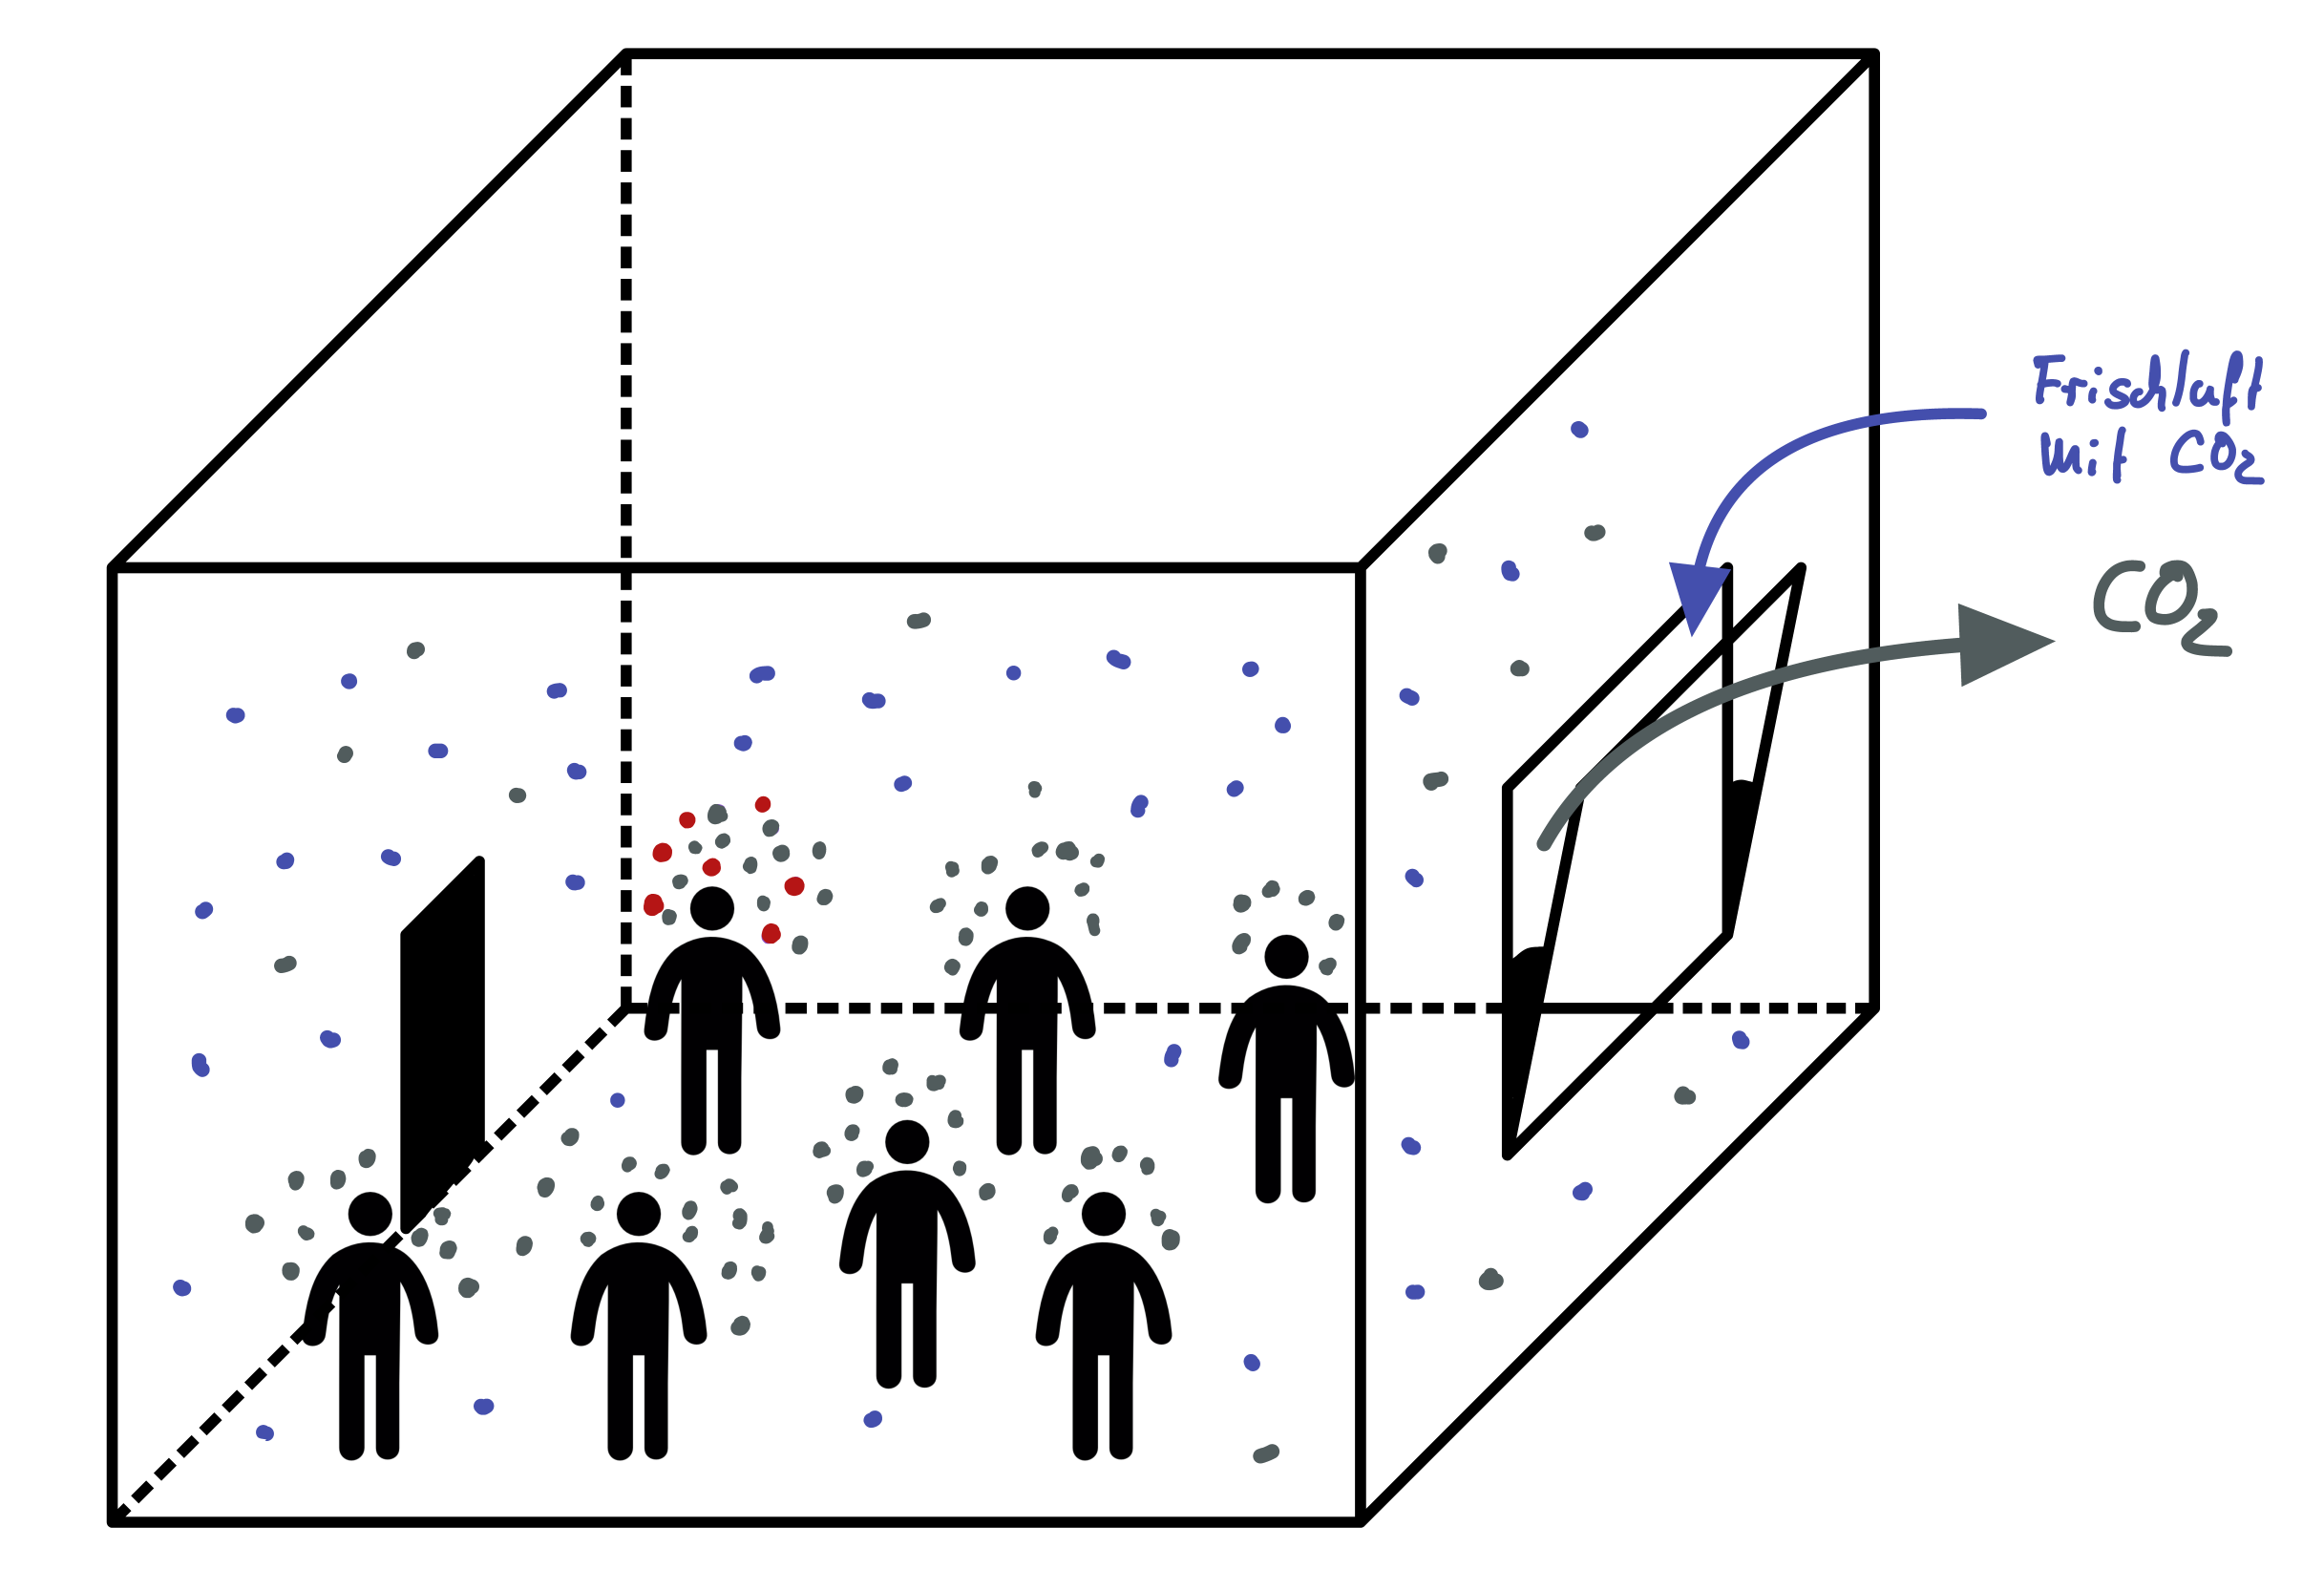
\includegraphics[width=1.\textwidth]{img/spaltluft}
		\end{minipage}
	\begin{minipage}{0.45 \textwidth}
			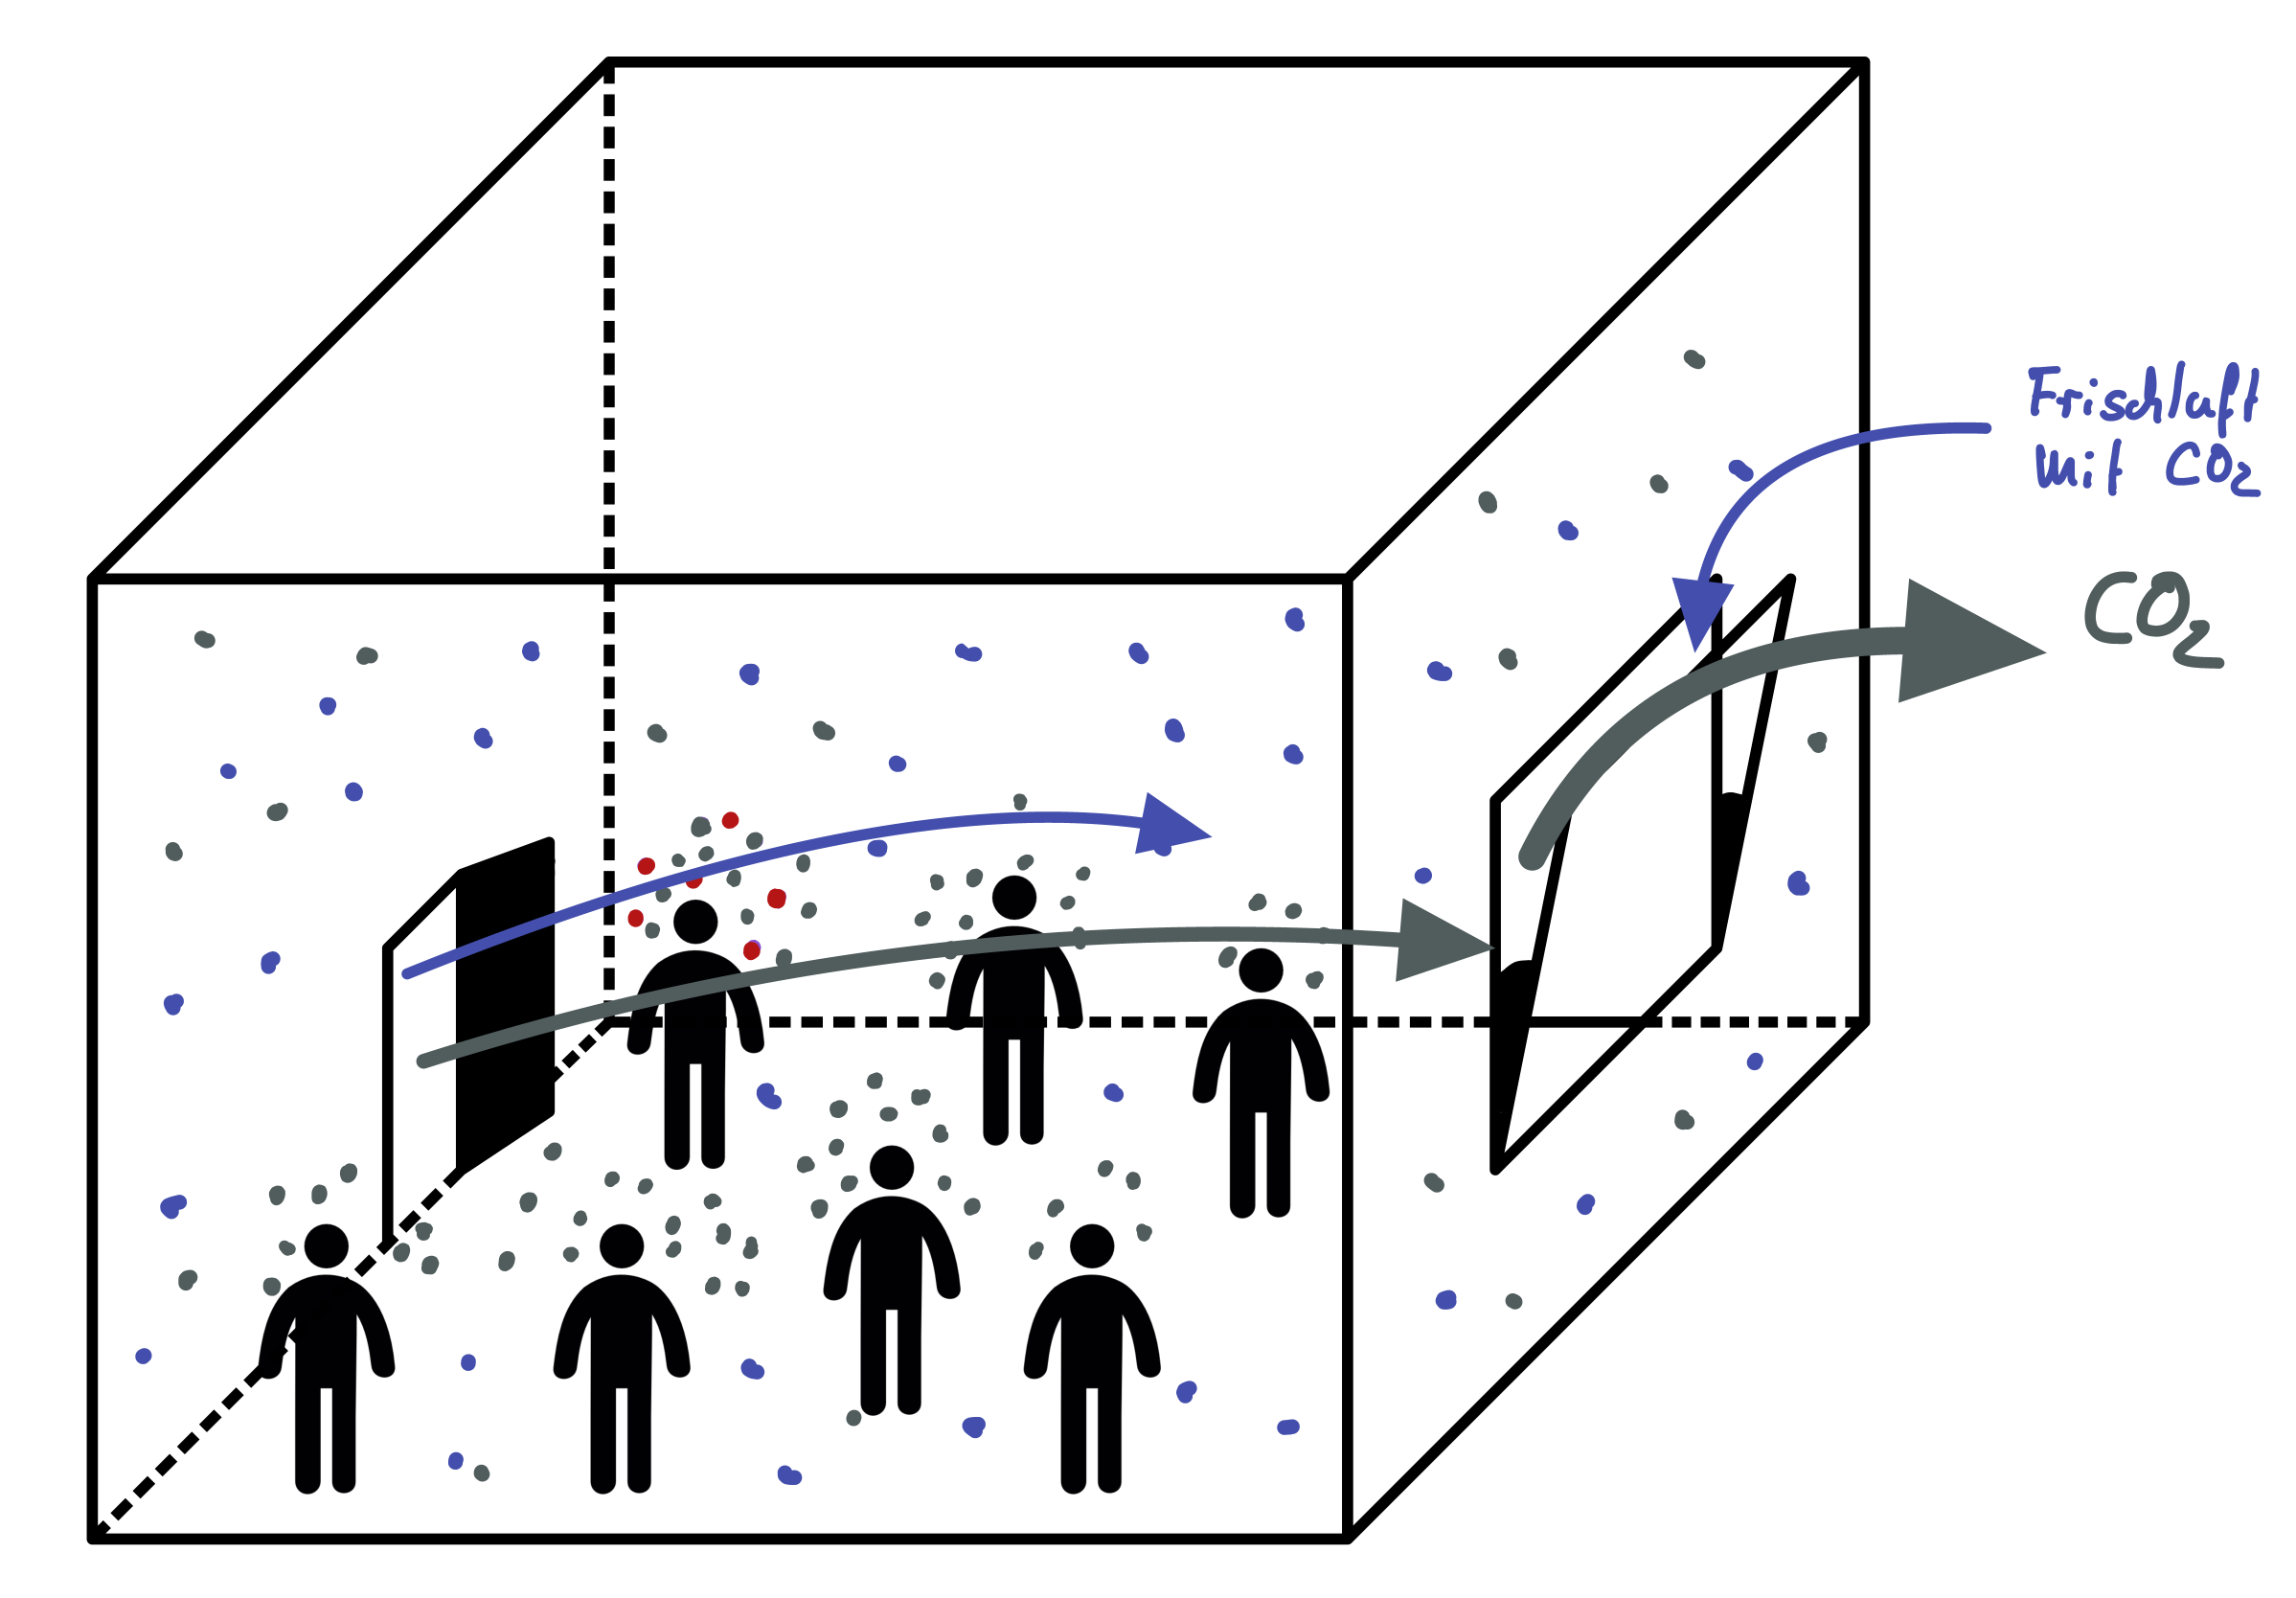
\includegraphics[width=1.\textwidth]{img/querluft}
	\end{minipage}
	\caption{Spaltluft- und Querluftströmung}
	\label{fig:querluft_spaltluft}
	\end{figure}
\FloatBarrier

\subsubsection*{Alkalisches Mauerwerk}
Auch das Mauerwerk kann für den CO2-Gehalt entscheidend sein, da dabei der verarbeitete Kalkmörtel (bestehend aus Sand, Löschkalk und Kies) zu Calciumcarbonat reagiert. 
\begin{flalign*}
	\ce{Ca(OH)2 + CO2 -> CaCO3 + H2O}
\end{flalign*}

